

\chapter{Chosen Ciphertext Security}

\section{Encryption and Authentication}	
	\begin{itemize}
		\item ...are different goals...
		\item ...not always!
	\end{itemize}
	\begin{center}
		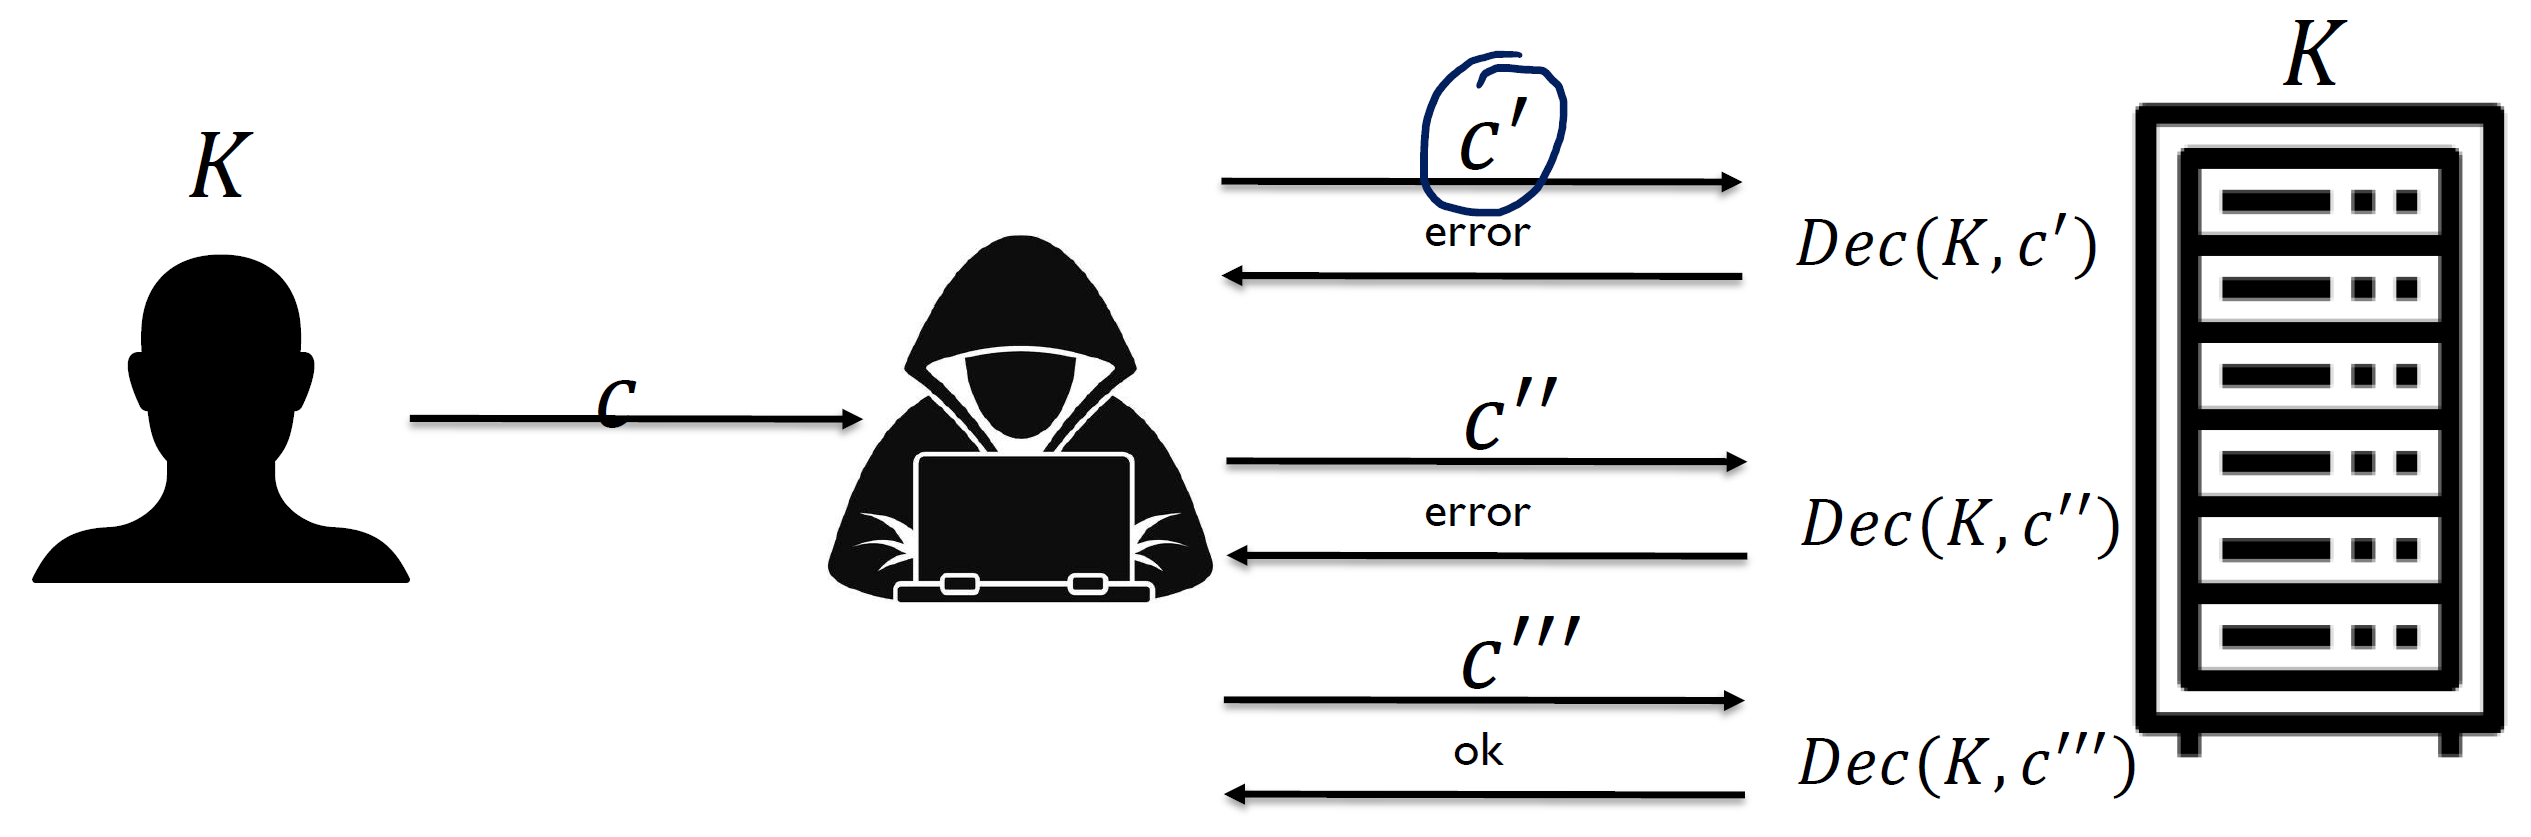
\includegraphics[width=110mm]{Graphics/Chosen Ciphertext Security/ccs1.png}
	\end{center}

	\begin{definition}[$IND-CCA$-secure]
		An encryption scheme $(KeyGen,Enc,Dec)$ is indistinguishable under chosen ciphertext attacks, or $IND-CCA$\textbf{-secure}, 
		if it holds for \textbf{every PPT-bounded adversary} $\mathcal{A}$ there exists a negligible function $v$ s.t. for all $\lambda \in \mathbb{N}$
		$$Pr[IND-CCA_{\mathcal{A}}(\lambda) = 1] < \frac{1}{2} + v(\lambda)$$
	\end{definition}
	\begin{center}
		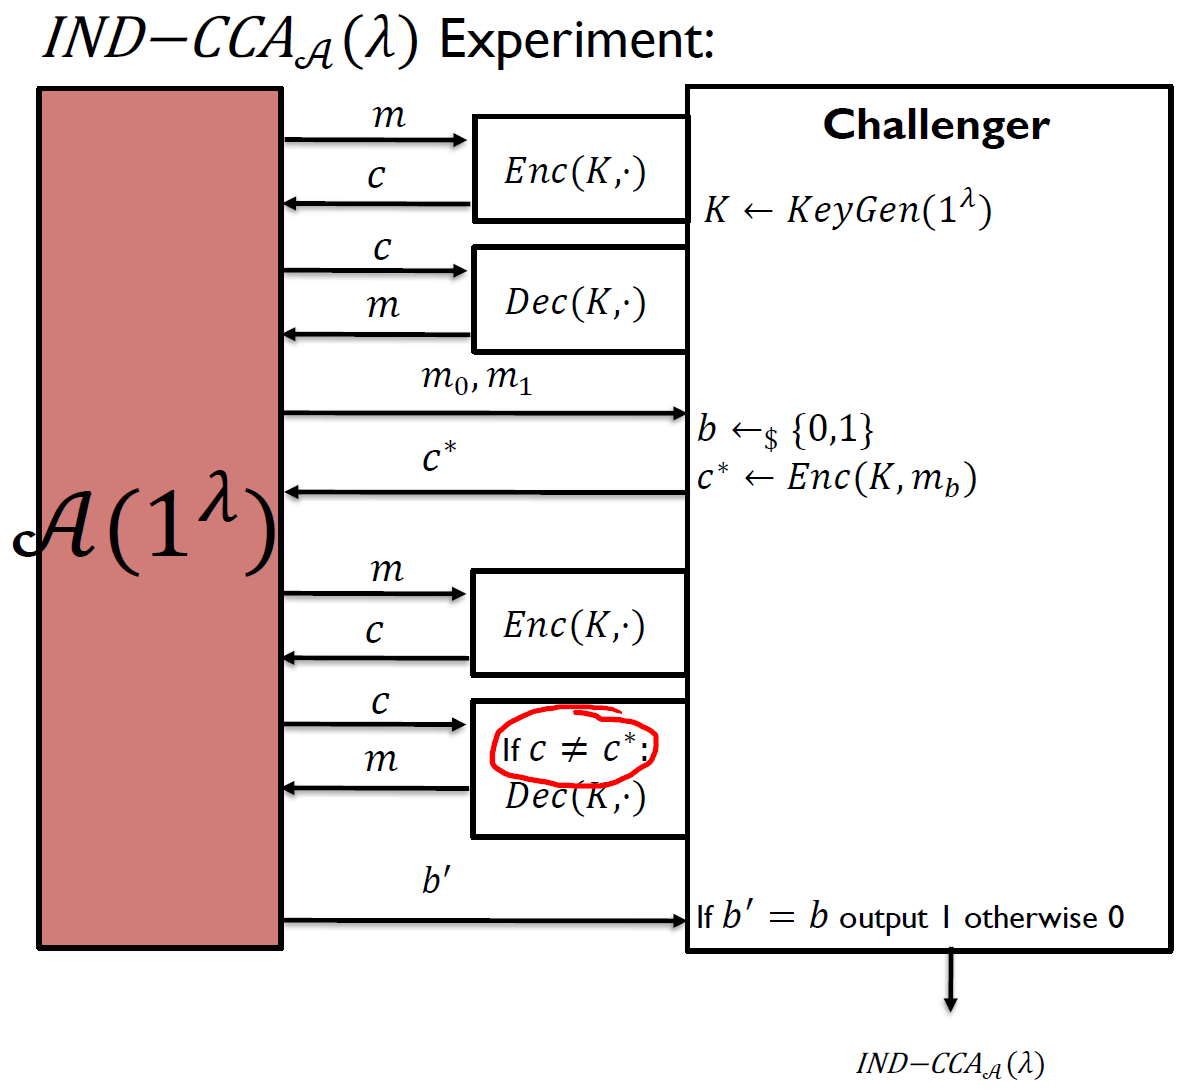
\includegraphics[width=110mm]{Graphics/Chosen Ciphertext Security/ccs2.png}
	\end{center}
	
\section{Constructing $IND-CCA$ secure encryption}
	\begin{itemize}
		\item Idea: Use authentication
		\item But how?
		\item 3 Options:
		\begin{enumerate}
			\item Authenticate and Encrypt: $Enc(K_1,m),Mac(K_2,m)$
			\item Authenticate then Encrypt: $Enc(K_1,(m||Mac(K_2,m)))$
			\item Encrypt then Authenticate: $Enc(K_1,m),Mac(K_2,Enc(K_1,m))$
		\end{enumerate}
		\item Evaluation of the 3 options:
		\begin{enumerate}
			\item Authenticate and Encrypt: $Enc(K_E,m),Mac(K_M,m)$\\
				$\Rightarrow$ Is bad: $Mac(K_M,m) = (Mac'(K_M,m),m)$
			\item Authenticate then Encrypt: $Enc(K_E,(m||Mac(K_M,m)))$\\
				$\Rightarrow$ Also bad: $Enc(K_E,m) = (Enc'(K_E,m),r)$
			\item Encrypt then Authenticate: $Enc(K_E,m),Mac(K_M,Enc(K_E,m))$\\
				$\Rightarrow$ Winner!
		\end{enumerate}
	\end{itemize}

	\textbf{Construction 6.4:}
	Let $(KeyGen,Enc,Dec)$ be an encryption scheme and\\
	$(Gen,Mac,Verify)$ a $MAC$.
	\begin{itemize}
		\item $KeyGen'(1^{\lambda})$: Compute $K_E \leftarrow KeyGen(1^{\lambda})$ and $K_M \leftarrow Gen(1^{\lambda})$ and output $K \leftarrow (K_E,K_M)$.
		\item $Enc'(K,m)$: Parse $K = (K_E,K_M)$.
			Compute $c \leftarrow Enc(K_E,m)$ and $t \leftarrow Mac(K_M,c)$.
			Output $c' \leftarrow (c,t)$.
		\item $Dec'(K,c')$: Parse $K = (K_E,K_M)$ and $c' = (c,t)$.\\
			If $Verify(K_M,c,t) = 1$ output $m \leftarrow Dec(K_E,c)$, otherwise $\bot$
	\end{itemize}
	\textbf{Correctness:}
	Follows from correctness of $(KeyGen,Enc,Dec)$ and $(Gen,Mac,Verify)$.
	
	\begin{theorem}\label{thm6.5}
		If $(KeyGen,Enc,Dec)$ is an $IND-CPA$ secure encryption scheme and $MAC = (Gen,Mac,Verify)$ is a $sEUF-CMA$ secure message authentication code, 
		then $(KeyGen',Enc',Dec')$ is an $IND-CCA$ secure encryption scheme.
	\end{theorem}
	\begin{proof}
		Assume $(KeyGen',Enc',Dec')$ is not an $IND-CCA$ secure encryption scheme!\\
		$\Rightarrow$ $(KeyGen,Enc,Dec)$ is not $IND-CPA$ secure or $(Gen,Mac,Verify)$ is not $sEUF-CMA$ secure.\\
		Thus, assume there is a PPT-adversary $\mathcal{A}$ and a non-negligible $\epsilon$ so that
		$$Pr[IND-CCA_{\mathcal{A}}(\lambda) = 1] > \frac{1}{2} + \epsilon$$
		We call $Exp$ the $IND-CCA_{\mathcal{A}}(\lambda)$ experiment.
		\begin{center}
			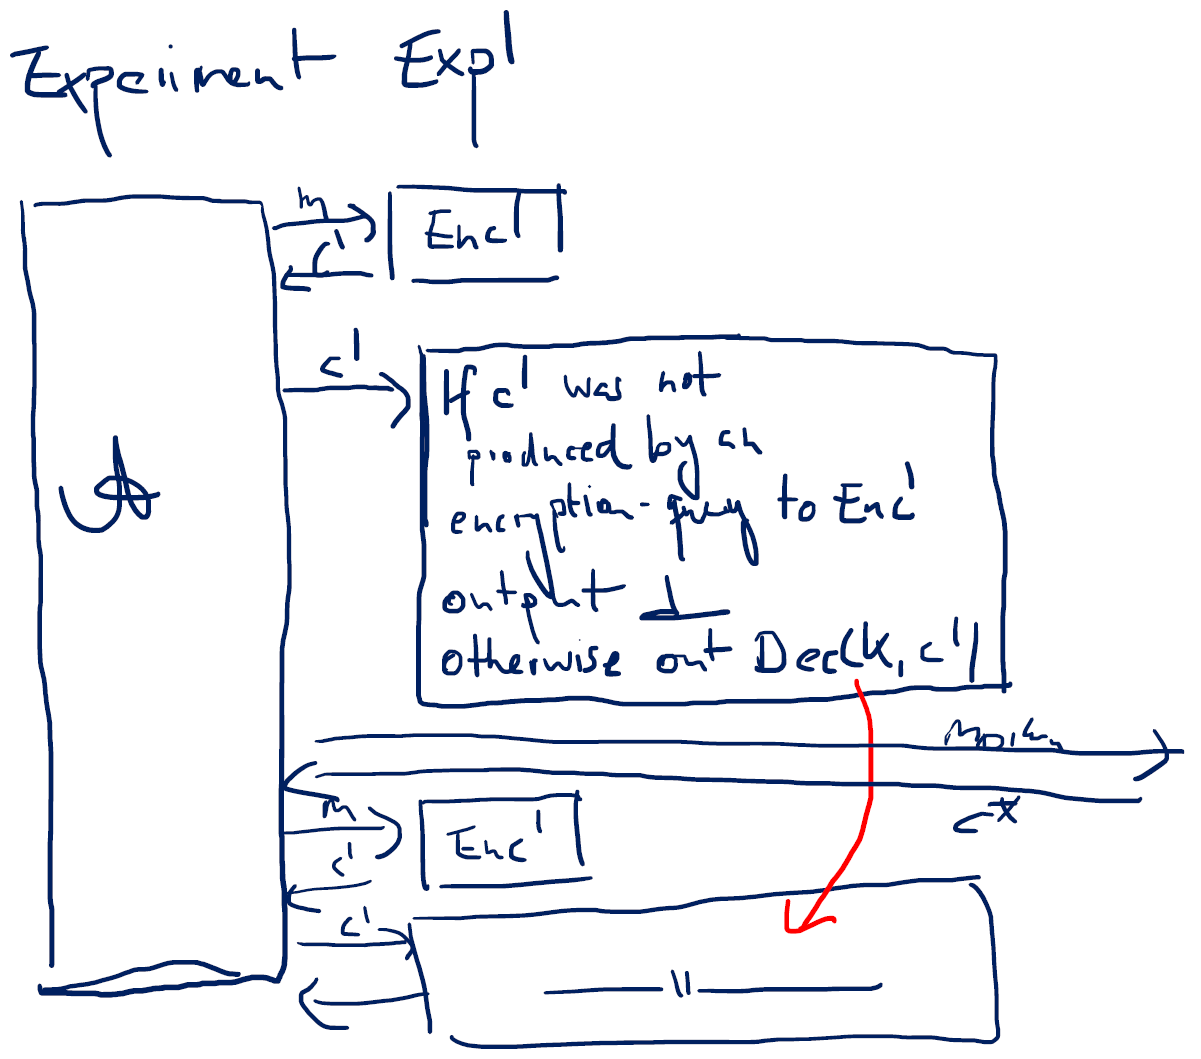
\includegraphics[width=80mm]{Graphics/Chosen Ciphertext Security/ccs3.png}
		\end{center}
		\underline{\textbf{Claim:}}
		$$|Pr[Exp=1]-Pr[Exp'=1]| > \epsilon'$$
		for a non-negligible $\epsilon'$\\
		$\Rightarrow$ $(Gen,Mac,Verify)$ is not $sEUF-CMA$ secure.\\\\
		\underline{Proof of Claim:}
		Let $ValidQuery$ (short: $VQ$) be the event that $\mathcal{A}$ sends a decryption query $c' = (c,t)$ with
		$Verify(K,m,c,t) = 1$ but $c'$ was not obtained by an encryption query.\\
		Conditioned on $\overline{ValidQuery}$ (short: $\overline{VQ}$) $\Rightarrow$ $Exp$ and $Exp'$ behave identically.\\
		So it follows with LOTP that
		\begin{enumerate}
			\item $Pr[Exp=1] = Pr[Exp=1 \mid VQ] \cdot Pr[VQ] + Pr[Exp=1 \mid \overline{VQ}] \cdot Pr[\overline{VQ}]$
			\item $Pr[Exp'=1] = Pr[Exp'=1 \mid VQ] \cdot Pr[VQ] + Pr[Exp'=1 \mid \overline{VQ}] \cdot Pr[\overline{VQ}]$
		\end{enumerate}
		With $Pr[Exp=1 \mid \overline{VQ}] \cdot Pr[\overline{VQ}] = Pr[Exp'=1 \mid \overline{VQ}] \cdot Pr[\overline{VQ}]$ it follows that
		$$\epsilon' < |Pr[Exp=1]-Pr[Exp'=1]| = |Pr[Exp=1 \mid VQ]-Pr[Exp'=1 \mid VQ]| \cdot Pr[VQ] \leq Pr[VQ] \text{,}$$
		because $|Pr[Exp=1 \mid VQ]-Pr[Exp'=1 \mid VQ]| \leq 1$.\\
		Construct an adversary $\mathcal{A}'$ against $sEUF-CMA$ security of $(Gen,Mac,Verify)$ with non-negligible success probability.\\
		$\mathcal{A}$ makes at most $q$ decryption queries.
		\begin{center}
			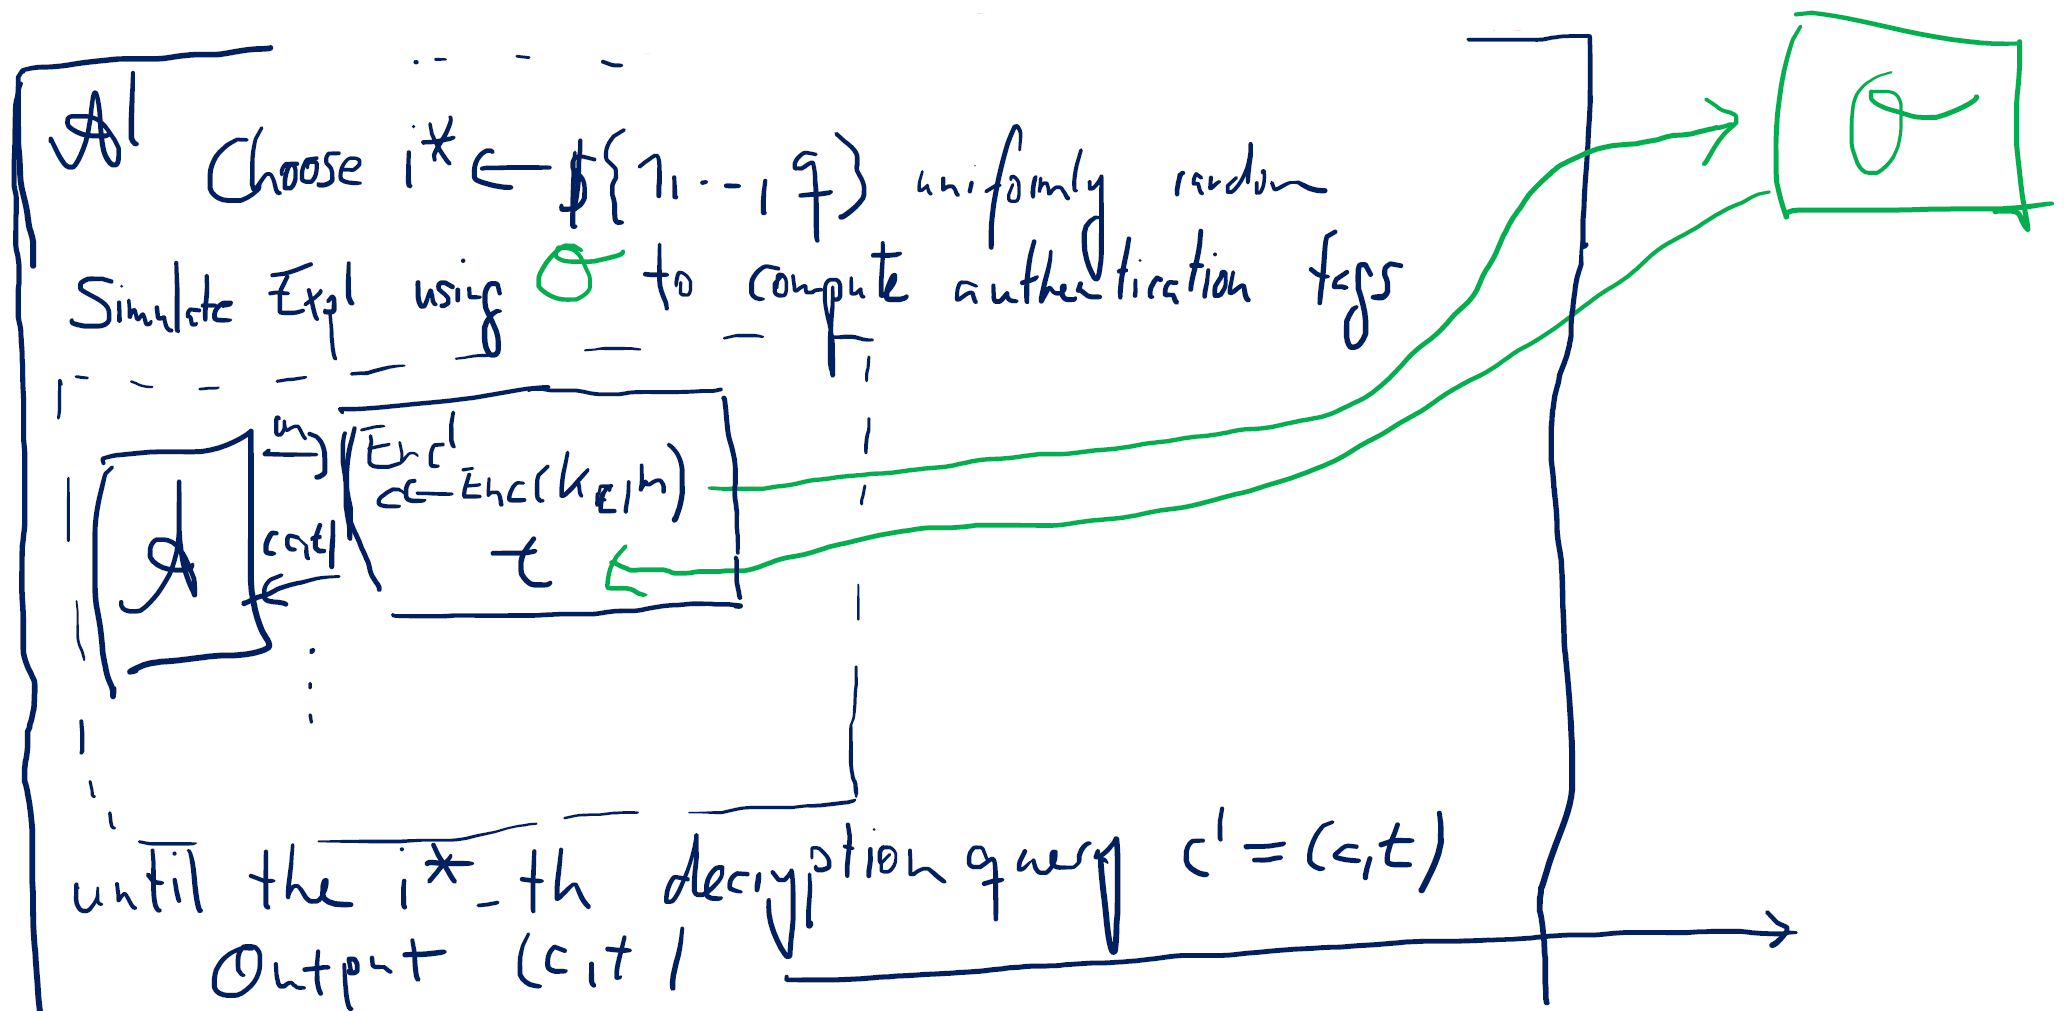
\includegraphics[width=160mm]{Graphics/Chosen Ciphertext Security/ccs4.png}
		\end{center}
		\begin{itemize}
			\item From view of $\mathcal{A}$, $Exp'$ and $\mathcal{A}'s$ simulation are identical.
			\item If $ValidQuery$ occurs, then there is an index $i \in \{1,...,q\}$ s.t. the $i$-th decryption query $c' = (c,t)$ 
			was \underline{not} produced by the encryption oracle and $Verify(K_M,c,t)=1$.
			\item Since $i^*$ is chosen uniformly random from $\{1,...,q\}$ it holds $Pr[i^* = i] = \frac{1}{q}$.
			\item If $ValidQuery$ happens and $i^* = i$ then $\mathcal{A}'$ outputs a new forge for the message $c$.
		\end{itemize}
		$\Rightarrow$ $Pr[sEUF-CMA_{\mathcal{A}'}(\lambda) = 1] \geq Pr[i^* = i \  \text{and} \  VQ] = Pr[i^* = i] \cdot Pr[VQ] \geq \frac{1}{q} \cdot \epsilon' = \frac{\epsilon'}{q}$
		non-negligible.\\
		But this contradicts the $sEUF-CMA$ security of $MAC$! Thus
		$$|Pr[Exp=1]-Pr[Exp'=1]| < negl \Rightarrow Pr[Exp'=1] > \frac{1}{2} + \epsilon - negl$$
		with $\epsilon'' = \epsilon - negl$ which is non-negligible!
\newpage
		Construct a PPT adversary $\mathcal{A}''$ against $IND-CPA$ security of $(KeyGen,Enc,Dec)$ with advantage $\epsilon''$
		\begin{center}
			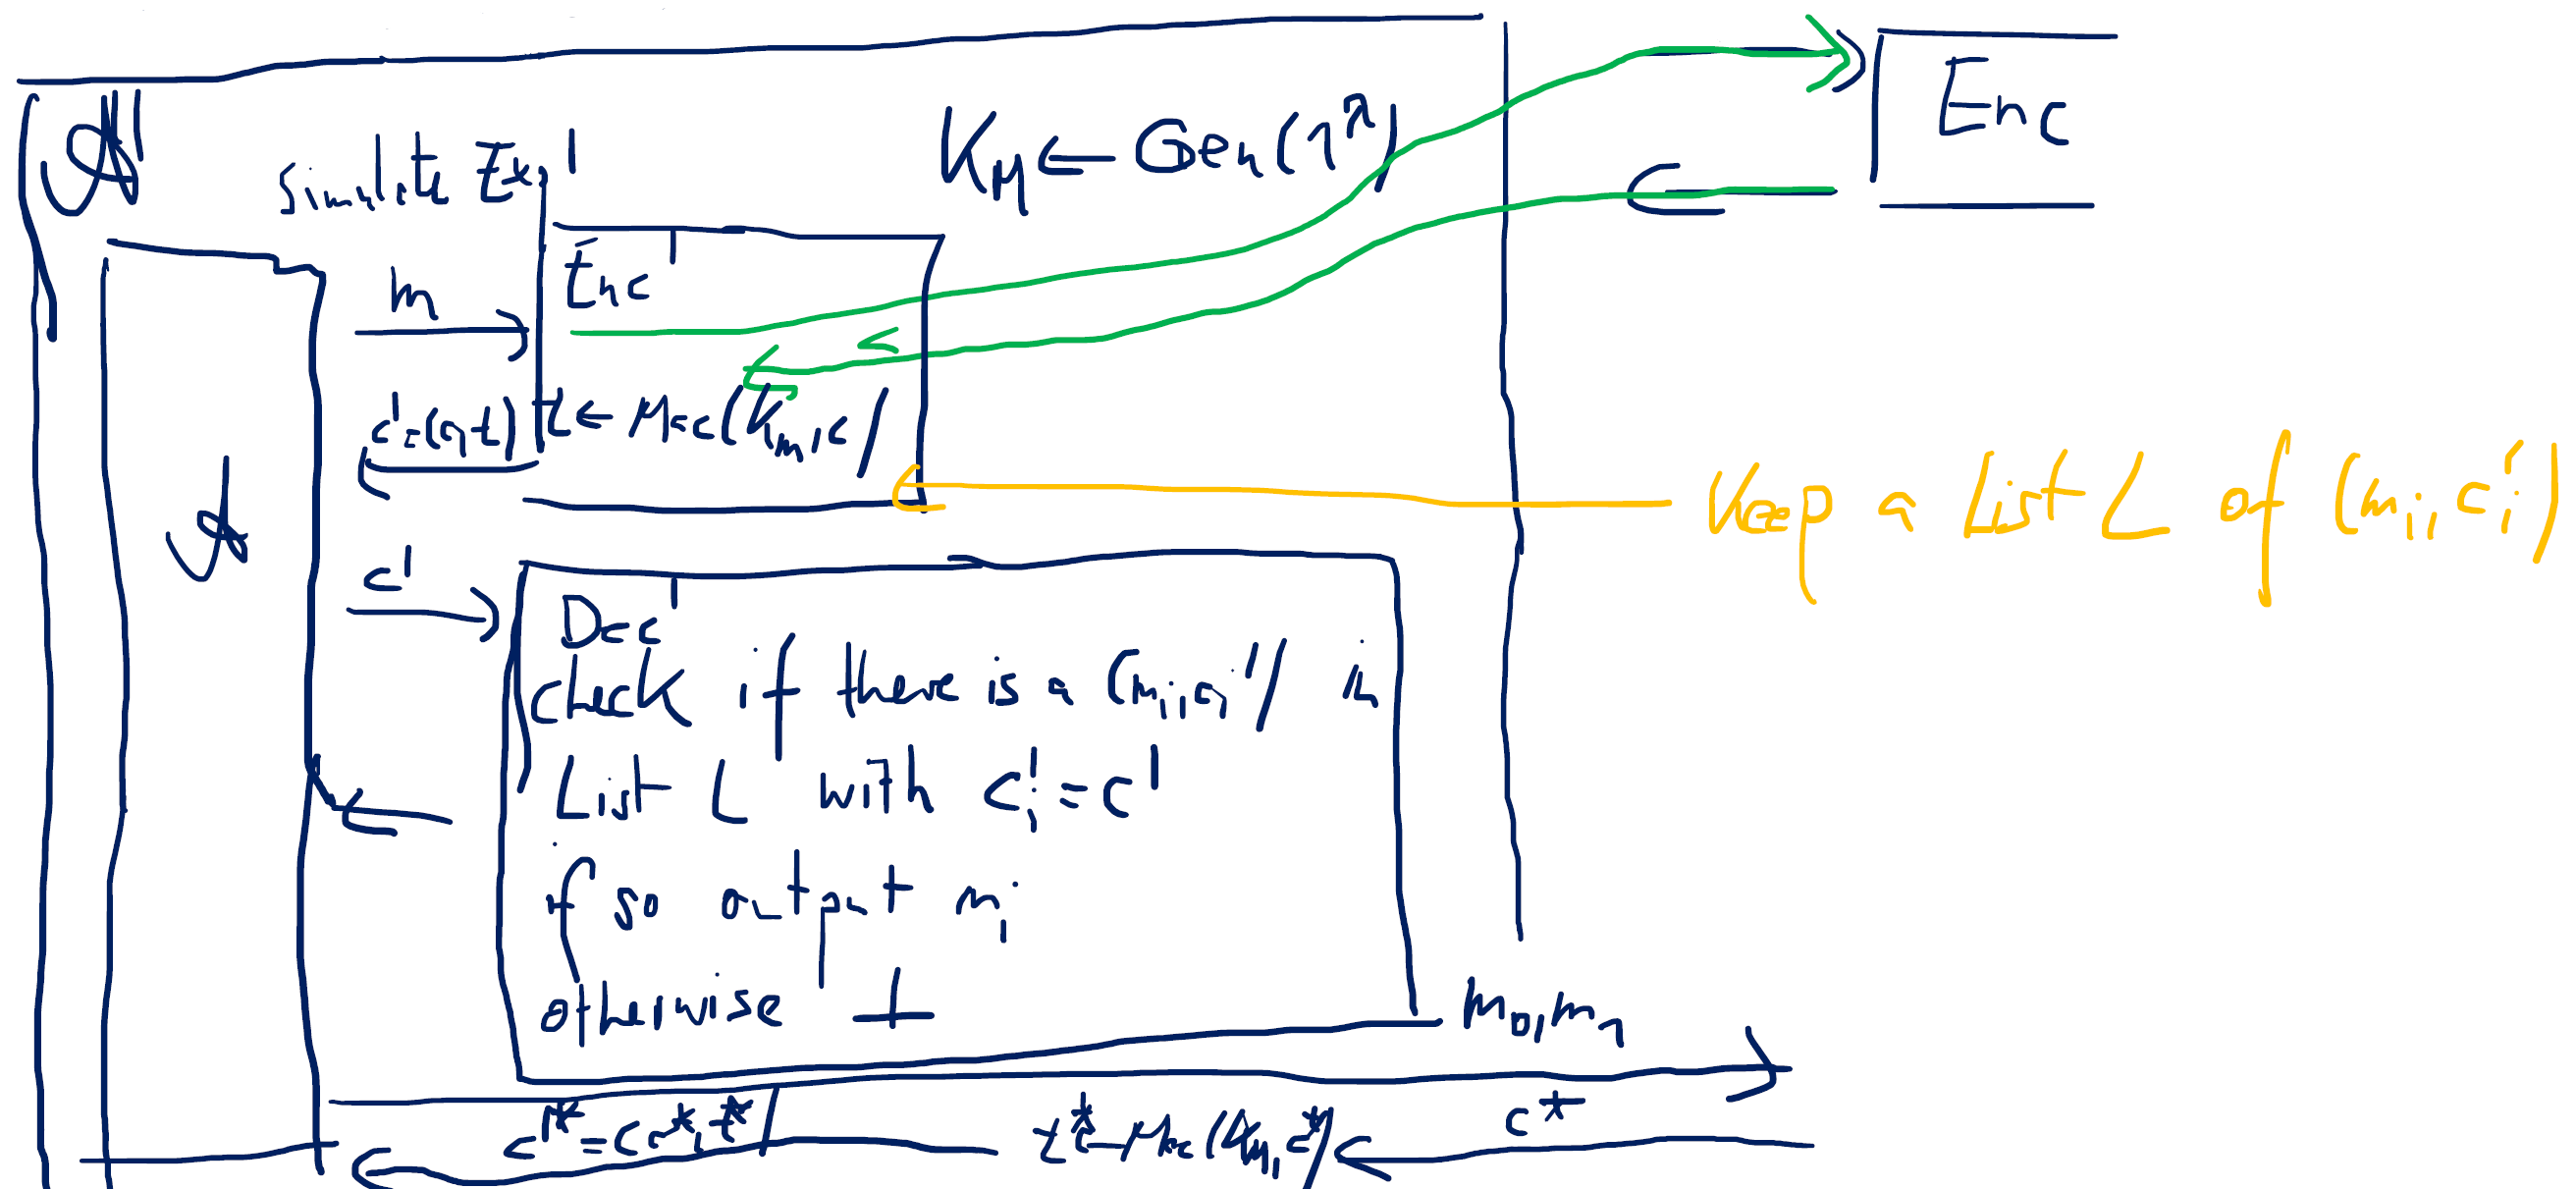
\includegraphics[width=160mm]{Graphics/Chosen Ciphertext Security/ccs5.png}
		\end{center}
		From view of $\mathcal{A}$, $Exp'$ and simulation by $\mathcal{A}'$ are identically distributed
		\begin{itemize}
			\item[->] $Enc'$ oracles behave identically.
			\item[->] $Dec'$ oracles behave identically given that $(KeyGen,Enc,Dec)$ is correct.
		\end{itemize}
		$\Rightarrow$ $Pr[IND-CPA_{\mathcal{A}''}(\lambda)=1] = Pr[Exp'=1] > \frac{1}{2} + \epsilon''$\\
		$\Rightarrow$ This contradicts $IND-CPA$ security of $(KeyGen,Enc,Dec)$!
	\end{proof}

\section{Summary}
	\begin{itemize}
		\item Active adversaries try to break secrecy by manipulating messages and observing behavior other parties
		\item $IND-CCA$ security provides security against active adversaries
		\item Modeled by giving the adversary access to a decryption oracle
		\item $IND-CCA$ encryption from $IND-CPA$ encryption and $MAC$ via encrypt-then-mac!
	\end{itemize}
	

